%
% chapter.tex -- Krümmung
%
% (c) 2025 Prof Dr Andreas Müller
%
\chapter{Krümmung
\label{chapter:kruemmung}}
\kopflinks{Krümmung}
In Abbildung~\ref{buch:kruemmung:fig:exzess}
%
% fig-exzess.tex
%
% (c) 2025 Prof Dr Andreas Müller
%
\begin{figure}
\centering
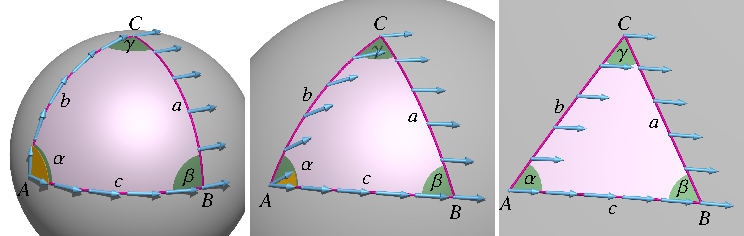
\includegraphics{chapters/110-kruemmung/images/exzess.pdf}
\caption{Der Paralleltransport eines Tangentialvektors um ein 
sphärisches Dreieck führt wegen der Krümmung der Kugeloberfläche
zu einer Drehung des Vektors um den orangen Winkel beim Punkt $A$.
Für kleine Dreiecke bzw.~grosse Kugelradien nähert sich das
Dreieck einem ebenen Dreieck an und die Drehung wird sehr klein.
\label{buch:kruemmung:fig:exzess}}
\end{figure}

%
% fig-drehung.tex
%
% (c) 2025 Prof Dr Andreas Müller
%
\begin{figure}
\centering
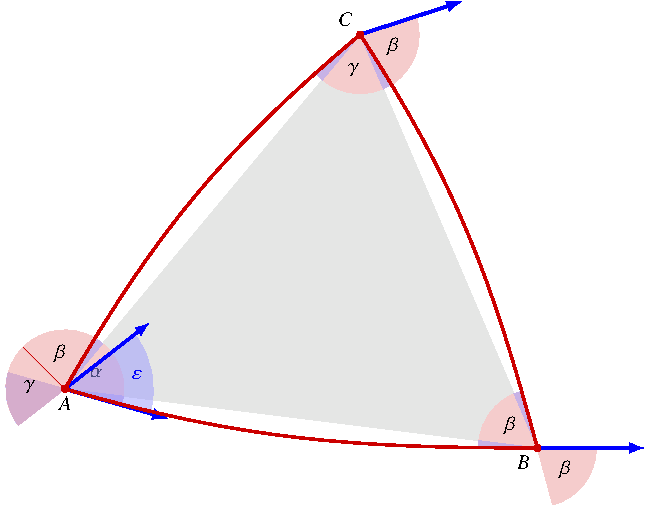
\includegraphics{chapters/110-kruemmung/images/drehung.pdf}
\caption{Die Drehung eines Vektors beim Paralleltransport eines
Tangentialvektors ausgehend vom Punkt $A$ entlang der Seiten eines
sphärischen Dreiecks entlang der Seiten des Dreiecks resultiert
in einer Drehung um den blauen Winkel.
Er ist gleich gross wie die Summe der in jeder Ecke eingezeichneten
kleinen blauen Winkel, die anzeigen, wieviel grösser die Winkel
des sphärischen Dreiecks sind als die des ebenen Dreiecks
$\triangle ABC$.
Ihre Summe heisst daher der sphärische Exzess
$\varepsilon = \alpha+\beta+\gamma-\pi$.
\label{buch:kruemmung:fig:drehung}}
\end{figure}

sind gleichseitige sphärische Dreiecke zu unterschiedlichen
Kugelradien dargestellt.
Die Seiten $a=b=c$ sind gleich, ebenso die Winkel $\alpha=\beta=\gamma$.
Das Dreieck ganz rechts ist im Vergleich zum Kugelradius so klein,
dass die Krümmung kaum mehr sichtbar ist.
Nach dem Seitenkosinussatz
\[
\cos c = \cos a\cos b + \sin a \sin b \cos\alpha
\]
der sphärischen Trigonometrie folgt für das gleichseitige Dreieck
\begin{align*}
\cos a-\cos^2a
&=
\sin^2 a \cos\alpha
=
(1-\cos^2 a)\cos\alpha
\\
\cos a(1-\cos a)
&=
(1+\cos a)(1-\cos a)\cos\alpha
\intertext{und nach Division durch $1-\cos a$}
\frac{ \cos a }{ 1+\cos a }
&=
\cos\alpha.
\end{align*}
Im Grenzwert $a\to 0$ strebt $\cos a$ gegen 1.
Der Grenzwert für den Winkel $\alpha$ ergibt sich daher aus
$\cos\alpha=\frac12$ als $\alpha=60^\circ$.

Der Transport des Tangentialvektors entlang der Seite $AB$ eines
beliebigen sphärischen Dreiecks wie in
Abbildung~\ref{buch:kruemmung:fig:drehung}
liefert den Tangentialvektor an $AB$ im Punkt $B$.
Dieser schliesst mit der Seite $BC$ den Winkel $\beta$ ein.
Der Paralleltransport dieses Vektors ergibt einen Vektor im Punkt $C$,
der mit der Seite $CA$ einen Winkel $\beta+\gamma$ einschliesst.
Durch Paralleltransport zum Punkt $A$ ergibt sich eine Drehung um
insgesamt $\varepsilon= \alpha+\beta+\gamma -\pi$.
Die Grösse $\varepsilon$ ist bekannt als der {\em sphärische Exzess}
\index{Exzess, sphärisch}%
\index{sphärischer Exzess}%
Bei einem ebenen Dreieck verschwindet der sphärische Exzess,
beim Paralleltransport eines Vektors ist keine Drehung feststellbar.

Beim gleichseitigen sphärischen Dreieck von
Abbildung~\ref{buch:kruemmung:fig:exzess}
sind alle Winkel gleich gross, der sphärische Exzess und damit die
Drehung des Tangentialvektors ist daher $\varepsilon=3\alpha-\pi$. 
Er erreicht für ein Dreieck mit drei rechten Winkeln und drei
Seiten der Längen $\frac{\pi}2$ den Wert $\frac{\pi}2$.

Der sphärische Exzess eines sphärischen Dreiecks ist auch ein Mass für
den Flächeninhalt $\Delta F = (\alpha+\beta+\gamma-\pi)R^2$.
Je grösser der Flächeninhalt in Relation zur Oberfläche der Kugel,
desto grösser die Drehung beim Paralleltransport eines Vektors um
ein Dreieck.
Oder je grösser der Drehwinkel, desto grösser die Krümmung $1/R^2$
der Kugeloberfläche.
Die Krümmung einer Fläche kann also verallgemeinert werden als
der Grenzwert des Verhältnisses des Drehwinkels eines Vektors um einen
geschlossenen polygonalen Weg zum Flächeninhalt des Polygons für
sehr kleine Polygone.

In Abschnitt~\ref{buch:kruemmung:section:riemann} dieses Kapitels
wird der riemannsche Krümmungstensor als eine lineare Abbildung,
die aus einem 2-Vektor eine Drehmatrix berechnet.
Zur Charakterisierung kann man aber auch nur einzelne Invarianten
der Drehmatrix verwenden.
Zum Beispiel lässt sich der Drehwinkel aus der Spur der Drehmatrix
berechnen.
Die Spur des riemannschen Krümmungstensors wird daher in 
Abschnitt~\ref{buch:kruemmung:section:riemann} als der Ricci-Tensor
eingeführt.
Aus dem Ricci-Tensor lassen sich die Einsteinschen Feldgleichungen
konstruieren, wie Abschnitt~\ref{buch:kruemmung:section:gravitation}
gezeigt wird.
Damit werden dann Aussagen über schwarze Löcher
(Abschnitt~\ref{buch:kruemmung:section:schwarzesloch})
und die Geschichte des Universums
(Abschnitt~\ref{buch:kruemmung:section:friedmann})
ableiten.

%
% Der riemannsche Krümmungstensor
%
\section{Berechnung der Krümmung
\label{buch:kruemmung:section:riemann}}
Das eingangs am Beispiel des Paralleltransports entlang eines
Dreiecksweges auf einer Kugeloberfläche illustrierte Phänomen
der Drehung eines paralleltransportierten Vektors soll jetzt
als Ausgangspunkt der Definition eines Krümmungsmasses sein.
Im Geiste der früheren Kapitel muss die Krümmung als eine 2-Form
beschrieben werden können, da die Krümmung offenbar durch Bewegung
entlang des Randes eines Flächenstücks erkennbar wird.
Allerdings können die Werte nicht nur skalare Werte sein, da
sich die Drehung eines Vektors nur mit Hilfe einer Matrix
beschreiben lässt.
Wir erwarten daher einen Tensor vierter Stufe.
Dieser Tensor ist der riemannsche Krümmungstensor.

%
% Der riemannsche Krümmungstensor
%
\subsection{Der riemannsche Krümmungstensor}
Das Einführungsbeispiel der Winkeldrehung eines paralleltransportieren
Vektors motiviert die Definition der Krümmung als die Abbildung 
der Tangentialvektoren beim Paralleltransport.
Ein Koordinatenparallelgramm mit den Ecken
\begin{center}
\begin{tikzpicture}[>=latex,thick]
\begin{scope}[xshift=-6cm,yshift=-0cm]
\node at (0,0) {$\displaystyle
\begin{aligned}
A &= x,\\
B &= x+\vec{h},\\
C &= x+\vec{h}+\vec{k}\\
\text{und}\quad
D &= x+\vec{k}
\end{aligned}$};
\end{scope}
\begin{scope}
\coordinate (A) at (-1.5,-1);
\coordinate (B) at (1.0,-0.5);
\coordinate (C) at (1.5,1);
\coordinate (D) at (-1.0,0.5);
\fill[color=gray!20] (A) -- (B) -- (C) -- (D) -- cycle;
\node at ($0.25*(A)+0.25*(B)+0.25*(C)+0.25*(D)$) {$\vec{h}\wedge\vec{k}$};
\draw[->] (A) -- (B);
\draw[->] (B) -- (C);
\draw[->] (C) -- (D);
\draw[->] (D) -- (A);
\fill (A) circle[radius=0.05];
\fill (B) circle[radius=0.05];
\fill (C) circle[radius=0.05];
\fill (D) circle[radius=0.05];
\node at (A) [below left] {$A$};
\node at (B) [below right] {$B$};
\node at (C) [above right] {$C$};
\node at (D) [above left] {$D$};
\node at ($0.5*(A)+0.5*(B)$) [below] {$\vec{h}$};
\node at ($0.5*(A)+0.5*(D)$) [left] {$-\vec{k}$};
\node at ($0.5*(B)+0.5*(C)$) [right] {$\vec{k}$};
\node at ($0.5*(D)+0.5*(C)$) [above] {$-\vec{h}$};
\end{scope}
\end{tikzpicture}
\end{center}
hat als Rand einen geschlossen Pfad, entlang dem ein Vektor parallel
transportiert werden soll.
Ein Vektor $A$ mit den Komponenten $a^i$ wird beim Transport entlang
des Weges linear abgebildet auf einen Vektor
$R(\vec{h}\wedge\vec{k})\cdot A$ abgebildet, der in linearer Näherung
nur vom 2-Vektor $\vec{h}\wedge\vec{k}$ und vom Vektor $A$ abhängt.
Der {\em riemannsche Krümmungstensor} ist daher die lineare Abbildung
\index{riemannscher Krümmungstensor}%
$R(\vec{h}\wedge\vec{k})$.

\subsubsection{Tangentialvektoren der Drehgruppen}
Der Krümmungstensor hängt antisymmetrisch von den Komponenten von
$\vec{h}$ und $\vec{k}$ ab und liefert eine Matrix, die von einer
Drehung herrührt.
Sei also $D(t)\in\operatorname{SO}(n)$ ein Weg in der Gruppe
der $n$-dimensionalen Drehmatrizen, die beim Parameterwert $t=0$
durch die Einheitsmatrix $I\in \operatorname{SO}(n)$ geht.
Er erfüllt
\begin{align*}
D(t)^tD(t) &= I
&&\text{und}&
\det D(t) &= 1.
\intertext{Die Ableitung nach $t$ an der Stelle $t=0$ ist}
\bigl(
\dot{D}(t)^tD(t)
+
D(t)^t\dot{D}^t
\bigr)\Bigl|_{t=0}
&=
0
&&\text{und}&
\operatorname{Spur}\dot{D}(0)
&=
0.
\end{align*}
Aus der linken Gleichung wird mit $D(0)=I$ die Bedingung
\[
\dot{D}(0) + \dot{D}(0)^t
\qquad\Rightarrow\qquad
\dot{D}(0)^t
=
-\dot{D}(0).
\]
Die Tangentialvektoren an die Drehgruppe sind als antisymmetrische
Matrizen mit verschwindender Spur.

\begin{beispiel}
Die Matrizen in der zweidimensionalen Drehmatrix sind
\[
D(t)
=
\begin{pmatrix}
\cos kt &          - \sin kt\\
\sin kt & \phantom{-}\cos kt
\end{pmatrix}
\]
mit der Ableitung
\[
\dot{D}(0)
=
\begin{pmatrix}
0 & -k\\
k &\phantom{-}0
\end{pmatrix}.
\qedhere
\]
\end{beispiel}

Die oben durchgeführten Rechnungen gelten nur in $\operatorname{SO}(n)$,
die mit dem Standardskalarprodukt definiert wird.
Auf einer beliebigen riemannschen Mannigfaltigkeit sind Drehmatrizen $D$
durch die Eigenschaft gegeben, dass
\[
D^t(t)GD(t)
=
G
\]
gilt.
Durch Ableitung nach $t$ an der Stelle $t=0$ folgt
\[
\dot{D}(0)^tG + G\dot{D}(0)
=
0
\qquad\Rightarrow\qquad
G\dot{D}(0)
=
-\dot{D}(0)^tG.
\]
Schreibt man die Komponenten von $\dot{D}(0)$ als $D^i\mathstrut_l$,
dann bedeutet dies
\[
g_{uv}D^{v}\mathstrut_l
=
-
\sum_{v}
D^{u}\mathstrut_v
g_{vl}
\]
Zieht man den oberen Index von $D^u\mathstrut_v$ mit herunter,
entsteht ein symmetrischer Tensor
\[
D_{uv}
=
g_{ui} D^i\mathstrut_v
\qquad\Rightarrow\qquad
D_{uv}
=
-D_{vu}.
\]

\subsubsection{Symmetrien des Krümmungstensors}
Der Krümmungstensor $R(\vec{h}\wedge\vec{k})$ hat als Wert eine Matrix,
deren Komponenten wir mit $R^i\mathstrut_l$ bezeichnen können.
Sie hängt antisymmetrisch von den Komponenten der beiden Vektoren
$\vec{h}\wedge\vec{k}$ ab.
In Komponenten ausgedrückt ist also
\[
R^i\mathstrut_l(\vec{h}\wedge\vec{k})
=
R^i\mathstrut_{luv} h^uk^v,
\]
wobei wie üblich nach der einsteinschen Summationskonvention über $u$
$v$ summiert werden muss.
Falls der metrische Tensor die Einheitsmatrix ist, muss $R^i\mathstrut_l$
antisymmetrisch sein, doch dies ist keine Eigenschaft, die allgemein
kovariant definiert ist.
Aus den Resultaten des letzten Abschnitts folgt aber, dass nach
Herunterziehen des oberen Index mithilfe von $g_{uv}$ eine
antismmetrische Matrix entsteht.
Für beliebige Vektoren $\vec{h}$ und $\vec{v}$ muss daher
$g_{li}R^i\mathstrut_l(\vec{h}\wedge\vec{k})=R_{il}(\vec{h}\wedge\vec{k})$
ein antisymmetrischer Tensor zweiter Stufe sein.
In Komponenten muss für beliebige Indizes $u$ und $v$ muss
$R_{jluv}=g_{ji}R^i\mathstrut_{luv}$ antisymmetrisch in den
Indizes $j$ und $l$ sein.

\subsubsection{Kovariante Ableitung und Krümmungstensor}
Wir berechnen jetzt den Paralleltransport des Vektors mit den
Komponenten $a^i$ entlang der Kantenpfade $ABC$ und $ADC$ 
des von $\vec{h}$ und $\vec{k}$ aufgespannten Parallelogramms.
Der Transport von $A$ nach $B$ ändert den Vektor um die Komponenten
\[
-\Gamma^l_{uv} a^u h^v 
\]
Der neue Vektor muss jetzt um den Vektor $\vec{k}$ transportiert
werden, der transportierte Vektor ist
\[
b^l
=
a^l-\Gamma^l_{uv} a^u h^v.
\]
Dies ergibt
\begin{align*}
\biggl(
\frac{\partial b^s}{\partial x^m}
+
\Gamma^s_{nm} b^n
\biggr)
k^m
&=
\biggl(
\frac{\partial \Gamma^s_{uv}}{\partial x^m}
a^u
h^v
-
\Gamma^s_{nm}
a^n
+
\Gamma^s_{nm} \Gamma^n_{uv}
a^u
h^v
\biggr)
k^m
\\
&=
\biggl(
\frac{\partial \Gamma^s_{uv}}{\partial x^m}
+
\Gamma^s_{nm}\Gamma^n_{uv}
\biggr)
a^u
h^v k^m
-
\Gamma^s_{nm}a^nk^m.
\end{align*}
Vertauschung von $v$ und $m$ führt auf den entsprechenden
Ausdruck für den Weg $ADC$.
Die Differenz ist der gesucht Krümmungstensor
\begin{align*}
R^s\mathstrut_{uvm}
&=
\frac{\partial\Gamma^s_{uv}}{\partial x^m}
-
\frac{\partial\Gamma^s_{um}}{\partial x^v}
-
\Gamma^s_{nm}\Gamma^n_{uv}
+
\Gamma^s_{nv}\Gamma^n_{um}
\end{align*}
Dies sind die Komponenten des riemannschen Krümmungstensors.
Durch herunterziehen des ersten Index erhält man die Komponenten
\[
R_{ruvm}
=
g_{rs}
\biggl(
\frac{\partial\Gamma^s_{uv}}{\partial x^m}
-
\frac{\partial\Gamma^s_{um}}{\partial x^v}
-
\Gamma^s_{nm}\Gamma^n_{uv}
+
\Gamma^s_{nv}\Gamma^n_{um}
\biggr)
\]
des kovarianten riemannschen Tensors.
Er ist antisymmetrisch in den ersten zwei und den letzten zwei
Indizes.

\begin{beispiel}
Der riemannsche Krümmungstensor für die Ebene in Polarkoordinaten.
\end{beispiel}

\begin{beispiel}
Der riemannsche Krümmungstensor für die Kugeloberfläche.
\end{beispiel}

\subsubsection{Herleitung mit Hilfe des Satzes von Green}
Für die Berechnung des Krümmungstensors haben wir ein konkretes
Parallelogramm verwendet und den Transport eines Vektors entlang
seiner Kanten approximiert.
Der Krümmungstensor ergab sich dann in linearer Näherung.
Dieser Zugang hat aber den Nachteil, dass er einen speziellen, nicht
differenzierbaren Weg und eine etwas holperig wirkende Approximation
verwendet, der Zulässigkeit nicht nachgeprüft wurde.

Der Satz von Green ermöglicht, ein Wegintegral über einen geschlossenen
Weg direkt zu formulieren und in ein Flächenintegral umzuwandeln.
Seien also $a^k$ die Komponenten eines Vektors $A$ und $\gamma(t)$ in
Weg mit den Koordinaten $x^i(t)$.
Der Vektor ändert beim Paralleltransport entlang der Kurve um den
Betrag $\Delta a^k$.
Die kovariante Ableitung $\nabla_{\dot{\gamma}} A$ gibt die infinitesimale
Änderung.
Die Änderung $\Delta a^k$ kann daher als das Integral
\begin{align*}
\Delta A
&=
\oint_{\gamma}
\nabla_{\dot{\gamma}}
A
\,d\gamma(t)
\intertext{über den Weg $\gamma$, oder in Komponenten}
\Delta a^k
&=
\int 
\biggl(
\frac{\partial a^k}{\partial x^v}
+
\Gamma^k_{uv} a^u
\biggr)
\dot{x}^v
\,dt.
\end{align*}
Um den Satz von Green anwenden zu können, brauchen wir ein ebenes
Kurvenintegral.
Wir betrachten daher einen Weg in der $x^v$-$x^s$-Koordinaten-Ebene.
Die Änderung entlang eines solchen Weges ist dann das Integral
\begin{align}
\Delta a^k
&=
\int
\biggl(
\frac{\partial a^k}{\partial x^v} + \Gamma^k_{uv}a^u
\biggr)
\,
dx^v
+
\biggl(
\frac{\partial a^k}{\partial x^s} + \Gamma^k_{us}a^u
\biggr)
dx^s,
\intertext{welches mit dem Satz von Green in das Integral}
&=
\int
\frac{\partial}{\partial x^s}
\biggl(
\frac{\partial a^k}{\partial x^v} + \Gamma^k_{uv}a^u
\biggr)
-
\frac{\partial}{\partial x^v}
\biggl(
\frac{\partial a^k}{\partial x^s} + \Gamma^k_{us}a^u
\biggr)
\,dx^u\,dx^s
\notag
\\
&=
\int
\frac{\partial^2 a^k}{\partial x^s\,\partial x^v}
-
\frac{\partial^2 a^k}{\partial x^v\,\partial x^s}
+
\frac{\partial \Gamma^k_{uv}}{\partial x^s} a^u
+
\Gamma^k_{uv}\frac{\partial a^u}{\partial x^s}
-
\frac{\partial \Gamma^k_{us}}{\partial x^v} a^u
-
\Gamma^k_{us}\frac{\partial a^u}{\partial x^v}
\,dx^v\,dx^s.
\label{buch:kruemmung:eqn:greendelta1}
\end{align}
Die zweiten Ableitungen heben sich weg und müssen daher nicht weiter
berücksichtigt werden.
Für den paralleltransportierten Vektor verschwindet die kovariante
Ableitung, so dass sie sich nach der partiellen Ableitung von $a^k$
nach den Koordinaten auflössen lässt.
Dies ergibt
\[
\frac{\partial a^u}{\partial x^s}
=
\Gamma^u_{sl}a^l.
\]
Eingesetzt in den Ausdruck
\eqref{buch:kruemmung:eqn:greendelta1}
ergibt sich
\begin{align*}
\Delta a^k
&=
\int
\frac{\partial\Gamma^k_{uv}}{\partial x^s} a^u
-
\frac{\partial\Gamma^k_{us}}{\partial x^v} a^u
+
\Gamma^k_{uv}\Gamma^u_{sl} a^l
-
\Gamma^k_{us}\Gamma^u_{vl} a^l
\,dx^s\,dx^v
\\
&=
\int
\biggl(
\frac{\partial\Gamma^k_{uv}}{\partial x^s}
-
\frac{\partial\Gamma^k_{us}}{\partial x^v}
+
\Gamma^k_{lv}\Gamma^l_{su}
-
\Gamma^k_{ls}\Gamma^l_{vu}
\biggr)
a^u
\,dx^s\,dx^v.
\end{align*}
Der Klammerausdruck im Integral ist wieder der riemannsche Krümmungstensor.

%
% Ricci-Krümmung
%
\section{Ricci-Krümmung
\label{buch:kruemmung:section:ricci}}
%
% fig-schnittkruemmung.tex
%
% (c) 2025 Prof Dr Andreas Müller
%
\begin{figure}
\centering
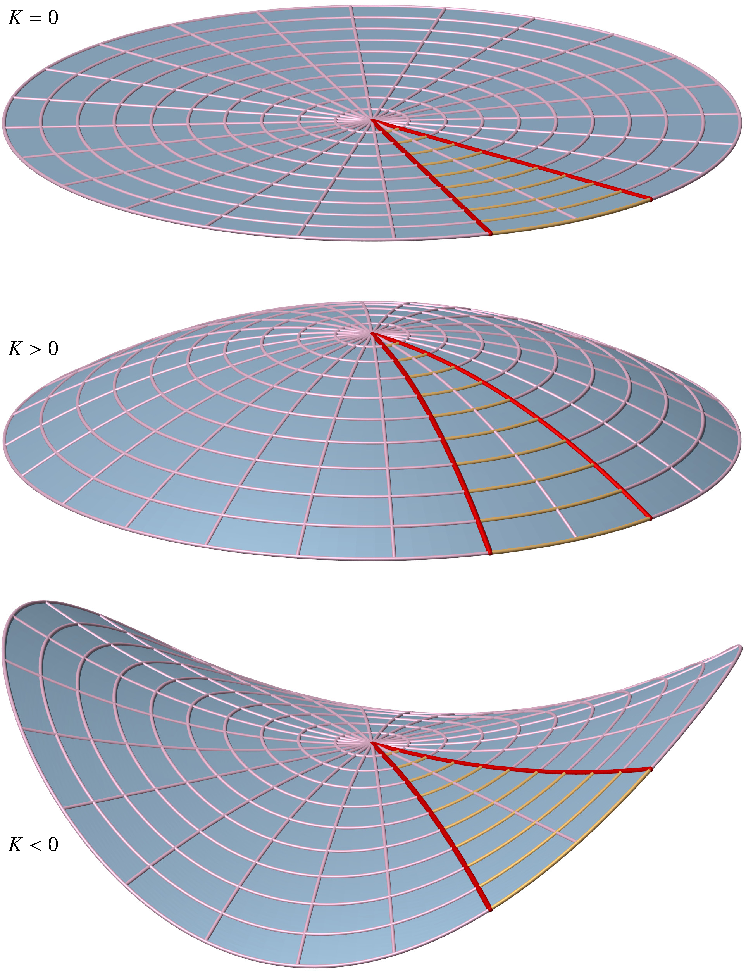
\includegraphics{chapters/110-kruemmung/images/kruemmung.pdf}
\caption{Die Schnittkrümmung bestimmt, wie schnell sich Geodäten
voneinander entfernen.
Der Abstand der Geodäten wächst linear mit dem Radius, wenn 
$K=0$ ist, der Abstand wächst schneller als linear für $K<0$ und
langsamer als linear für $K>0$.
\label{buch:kruemmung:fig:schnittkruemung}}
\end{figure}

Die Komponente $R^l\mathstrut_{ijk}$  des Riemann-Krümmungstensors
beschreibt, wie sich die $l$-Komponente des des $i$-ten 
Standardbasisvektors $\vec{e}_i$ beim Paralleltransport um
ein infinitesmales Quadrat mit dem 2-Vektor $\vec{e}_j\wedge \vec{e}_k$
verändert.
Für die physikalische Interpretation des Gravitationsfeldes ist
es wichtig zu verstehen, wie sich der Abstand von Geodäten mit
ähnlichen Anfangsbedingungen verändert, da wir dies als relative
Beschleunigung und damit als Anziehungs- oder Abstossungskraft 
interpretieren können.

%
% Schnittkrümmung
%
\subsection{Schnittkrümmung}
Wir betrachten zwei Geodäten mit initialem Tangentialvektor
$\vec{v}$, deren Anfangspunkte sich um eine kleine Verschiebung
in Richtung des Tangentialvektors $\vec{s}$ unterscheiden.

\begin{lemma}
Für die kovariante Ableitung zum Levi-Cività-Zusammenhang gilt
\[
\nabla_{\vec{v}}\nabla_{\vec{s}}\vec{v}
=
\nabla_{\vec{v}}\nabla_{\vec{v}}\vec{s}.
\]
\end{lemma}

\begin{proof}
Wir berechnen in Komponenten
Die Komponenten der Ableitungen der ersten kovarianten Ableitungen
sind
\begin{align*}
(\nabla_{\vec{s}}\vec{v})^i
&=
\biggl(
\frac{\partial v^i}{\partial x^k}
-
\Gamma^i_{kl} v^l
\biggr)
s^k
\\
(\nabla_{\vec{v}}\vec{s})^i
&=
\biggl(
\frac{\partial s^i}{\partial x^k}
-
\Gamma^i_{kl} s^l
\biggr)
v^k
\end{align*}

\end{proof}

\begin{align*}
\nabla_{\vec{v}}\nabla_{\vec{v}}\vec{s}
&=
-R(\vec{s}\wedge\vec{v})\cdot \vec{v}
\end{align*}
d.~h.~der Krümmungstensor gibt an, wie sich der
Verschiebungsvektor $\vec{s}$ zwischen den Geodäten ändert.

%
% Ricci-Krümmung
%
\subsection{Ricci-Krümmung}
Das Skalarprodukt
\begin{equation}
R(\vec{v},\vec{s})(\vec{v})\cdot\vec{s}
=
\langle
R(\vec{v}\wedge\vec{s})(\vec{v}) ,\vec{s}
\rangle_g
\label{buch:kruemmung:ricci:eqn:Rvsvs}
\end{equation}
ist ein Mass für die Änderung des Abstandes der Geodäten.
Es ist linear in allen Vektoren.
Aus den Symmetrieeigenschaften des riemannschen Krümmungstensors folgt
auch, dass es nur von $\vec{v}\wedge\vec{s}$ abhängt.
Multipliziert man $\vec{v}$ oder $\vec{s}$ mit einem Faktor $\lambda$,
wird  der Ausdruck \eqref{buch:kruemmung:ricci:eqn:Rvsvs} mit
$\lambda^2$, multipliziert.
Insbesondere ist
\[
K(\vec{s},\vec{v})
=
\frac{R(\vec{v}\wedge\vec{s})(\vec{v})\cdot\vec{s}}{|\vec{v}\wedge\vec{s}|^2}
\]
unabhängig von der Länge von $\vec{v}$ und $\vec{s}$.
Sie heisst die Schnittkrümmung.
Sie ist postiiv, wenn sich die Geodäten nähern und negativ, wenn sie
sich entfernen.

Ist $X$ ein Vektor mit den Komponenten $X^i$, dann ist
\[
R(\vec{e}_j\wedge X)(X)\cdot e_l
=
R^l\mathstrut_{ijk}X^iX^k.
\]
Für $l=j$ ergibt sich die Schnittkrümmung in der $\vec{e}_j$-$X$-Ebene.
Sie gibt die Änderung des Abstandes der Geodäten mit
Anfangsvektor $X$ an, wenn man den Anfangspunkt infinitesmal in
$\vec{e}_j$-Richtung verschiebt.

Die Summe
\begin{equation}
\sum_{j=1}^n
R(\vec{e}_j\wedge X)(X)\cdot \vec{e}_j
=
R^j\mathstrut_{ijk} X^iY^k
\label{buch:kruemmung:ricci:eqn:ricci}
\end{equation}
ist bis auf den Faktor $\frac1n$ der Mittelwert der Schnittkrümmungen
für die verschiedenen Differenzvektoren $\vec{s}=\vec{e}_j$.

\begin{definition}[Ricci-Krümmung]
\label{buch:kruemmung:ricci:def:ricci-kruemmung}
Der Tensor mit den Komponenten $R_{ik}=R^j\mathstrut_{ijk}$ heisst
der {\em Ricci-Krümmungstensor}.
Die Ricci-Krümmung zum Vektor $X$ ist
\[
\operatorname{Ric}(X,X)
=
\sum_{i,k=1}^n
\operatorname{Ric}(e_i,e_k)X^iX^k
=
R_{ik}X^iX^k.
\]
Sie ist eine quadratischer Form von $X$.
\end{definition}

Aus den Symmetrieeigenschaften des riemannschen Krümmungstensors folgt,
dass der Ricci-Tensor symmetrisch ist.

Die Konstruktion von $\operatorname{Ric}(X,X)$ als Summe über alle
Basisrichtungen ist ein richtungsunabhängiges Mass für die
Krümmung.
Positive Krümmung bedeutet, dass sich Geodäten im Mittel annähern.
Wir werden dies als gravitationelle Anziehungskraft interpretieren.
Wenn der Ricci-Tensor verschwindet, gibt es auch keine Gravitationskräfte.
Wir erwarten daher, dass es eine Feldgleichung gibt, die Masse und
Energie im Universum mit dem etwas spezielleren Ricci-Tensor verknüpft,
nicht mit dem ganz allgemeinen riemannschen Tensor.

%
% Krümmungsskalar
%
\subsection{Krümmungsskalar}
Die Spur des Ricci-Tensors
\[
R
=
g^{ik}R_{ik}
=
R^i_k
\]
heisst der {\em Krümmungsskalar}.
\index{Krümmungsskalar}
Der Krümmungsskalar ist also Tensor nullter Stufe eine weitere Invariante,
die in einer Feldgleichung für die Gravitation vorkommen könnte.

%
% Newtonsche Gravitation als Raumkrümmung
%
\section{Newtonsche Gravitation als Raumkrümmung
\label{buch:kruemmung:section:newton}}
Es gehört schon fast zum Allgemeinwissen, dass die einsteinsche
Relativitätstheorie die Gravitation als Raumkrümmung beschreibt.
Tatsächlich erlaubt aber auch die newtonsche Theorie eine solche
Interpretation, wie in diesem Abschnitt gezeigt werden soll.

%
% Koordinatensystem und newtonsche Gravitation
%
\subsection{Koordinatensystem und newtonsche Gravitation}
Wir verwenden ein vierdimensionales Koordinatensystem mit
den Koordinaten $x^0=ct$, $y^1=x$, $x^2=y$ und $x^3=z$.
Die Bahn eines Teilchens im Gravitationsfeld eines Himmelskörpers
der Masse $M$, der sich im Nullpunkt des Koordinatensystems befindet,
ist dann durch die Funktion
\[
t\mapsto
\begin{pmatrix}
ct\\
x(t)\\
y(t)\\
z(t)
\end{pmatrix}
\]
gegeben, die die Differentialgleichung
\begin{equation}
\frac{d^2}{dt^2}
\begin{pmatrix}
ct\\
x(t)\\
y(t)\\
z(t)
\end{pmatrix}
=
\begin{pmatrix}
0\\
\ddot{x}(t)\\
\ddot{y}(t)\\
\ddot{z}(t)
\end{pmatrix}
=
-
\frac{GMm}{r(t)^3}
\begin{pmatrix}
0\\
x(t)\\
y(t)\\
z(t)
\end{pmatrix}
\label{buch:kruemmung:newton:eqn:dgl}
\end{equation}
erfüllt, wobei
\[
r(t)
=
\sqrt{x(t)^2 + y(t)^2 + z(t)^2}
\]
ist.
Es ist möglich, die Bahn im Gravitationsfeld eines einzelnen,
ruhenden Himmelskörpers in geschlossener Form zu lösen.
Sobald mehrere massereiche Himmelskörper die Bahn beeinflussen,
wie dies im Sonnensystem mit dem Einfluss des Planeten Jupiter
der Fall ist, sind nur noch numerische Lösungen möglich.
Daher wird im folgenden nicht versucht, Lösungen direkt miteinander
zu vergleichen.
Stattdessen soll gezeigt werden, dass die Differentialgleichung
\eqref{buch:kruemmung:newton:eqn:dgl}
auch als Geodätengleichung einer geeigneten Metrik geschrieben
werden kann.
Zu diesem Zweck schreiben wir die Differentialgleichung noch in
der Komponentenform
\begin{equation}
\begin{aligned}
\ddot{x}^0(t) &= 0 \\
\ddot{x}^i(t) &= - \frac{GM}{r(t)^2}\,x^i(t)\qquad \text{für $i>0$}.
\end{aligned}
\label{buch:kruemmung:newton:eqn:dglcomponents}
\end{equation}
Die erste Gleichung bedeutet nichts anderes, als dass es in der
newtonschen Gravitationstheorie eine absolute Zeit gibt.

%
% Gravitationspotential
%
\subsection{Gravitationspotential}
Das newtonsche Gravitationsfeld ist ein Potentialfeld.
Das Potential der Masse $M$ im Nullpunkt des Koordinatensystems
hat das Potential
\[
U(x) = \frac{GM}{r}.
\]
Tatsächlich ist der Gradient 
\[
\operatorname{grad}U
=
-\frac{GM}{r^2} \operatorname{grad}{r}
=
-\frac{GM}{r^2}
\cdot
\frac{1}{2r}
\begin{pmatrix}
2x(t)\\
2y(t)\\
2z(t)
\end{pmatrix}
=
-\frac{GM}{r^3}
\begin{pmatrix}
x(t)\\
y(t)\\
z(t)
\end{pmatrix}
.
\]
Die rechte Seite stimmt mit der rechten Seite der Differentialgleichung
\eqref{buch:kruemmung:newton:eqn:dgl}
überein.

Sind mehrere Massepunkte gegeben, kann ihr gemeinsames Potential 
als Summe
\[
U(x)
=
\sum_{i=1}^n U_i(x)
\]
geschrieben werden, wobei
\[
U_i(x)
=
\frac{GM_i}{|x-x_i|}
\]
das Potential der Masse $M_i$ an der Stelle $x_i$ ist.

Für die folgende Rechnung gehen wir von der Annahme aus, dass sich die
Massen nicht bewegen, dass das Gravitationsfeld also statisch ist.
Diese Annahme ist näherungsweise dadurch gerechtfertigt, dass die
Geschwindigkeit der Massen in schwachen Gravitationsfeldern wie in
unserem Sonnensystem viel kleiner sind als die Lichtgeschwindigkeit.

%
% Metrik
%
\subsection{Metrik}
Wir verwenden die Metrik
\begin{equation}
\begin{aligned}
g_{00} &= \phantom{-}1 + \frac{2U(x)}{c^2} \\
g_{ii} &= -1\qquad &i&>0
\end{aligned}
\label{buch:kruemmung:newton:eqn:metrik}
\end{equation}
für die vierdimensionale Mannigfaltigkeit mit den Koordinaten
$(x^0,x^1,x^2,x^3)$.
Nur die Zeitkomponenten der Metrik weicht von der Minkowski-Metrik ab.

Da das Potential im Vergleich zu $c^2$ klein ist, werden wir nur in
erster Näherung arbeiten.
Terme zweiter Ordnung in $U/c^2$ enthalten Quadrate von $U/c^2$ und sind
noch viel kleiner, sie dürfen daher vernachlässigt werden.

In den folgenden Abschnitten werden schrittweise die Christoffel-Symbole
berechnet, mit denen dann in
Abschnitt~\ref{buch:kruemmung:newtion:subsection:geodaeten}
die Geodätengleichung aufgestellt werden soll.

%
% Die Inverse der Metrik
%
\subsubsection{Die Inverse der Metrik}
Da die Metrik im gewählten Koordinatensystem eine Diagonalmatrix ist,
ist auch die inverse Matrix diagonal mit den reziproken Diagonalelementen.
Wir brauchen nur eine Approximation in erster Ordnung in $2U/c^2$
für diese Elemente.

Das Element $g_{00}$ ist von der Form $1+x$.
Die geometrische Reihe
\[
1+q+q^2+q^3+\dots = \frac{1}{1-q}
\]
liefert für $q=-x$ die Approximation
\[
\frac{1}{1+x} = 1-x+x^2-x^3+o(x^3)
\]
für das reziproke Element.
Angewendet auf den Tensor $g_{ik}$ ergeben sich in erster Ordnung
die Diagonalelemente
\begin{equation}
\begin{aligned}
g^{00}
&=
\frac{1}{\displaystyle 1+\frac{2U}{c^2}}
=
1-\frac{2U}{c^2}+o\biggl(\frac{2U}{c^2}\biggr)
\\
g^{ii}&= -1
&&\text{für $i>0$.}
\end{aligned}
\end{equation}

%
% Ableitung der metrischen Koeffizienten
%
\subsubsection{Ableitungen der metrischen Koeffizienten}
Da nur das Element $g_{00}$ nicht konstant ist, gibt es nur die eine
nicht verschwindende Ableitung
\[
\frac{\partial g_{00}}{\partial x^k}
=
\begin{cases}
0
&\qquad\text{für $k=0$}\\[4pt]
\displaystyle
\frac{2}{c^2}
\frac{\partial U}{\partial x^k}
&\qquad\text{für $k>0$.}
\end{cases}
\]

%
% Christoffel-Symbole 1. Art
%
\subsubsection{Christoffel-Symbole erster Art}
Die Christoffel-Symbole erster Art sind
\[
\Gamma_{l,ik}
=
\frac{1}{2}\biggl(
\frac{\partial g_{lk}}{\partial x^i}
+
\frac{\partial g_{li}}{\partial x^k}
-
\frac{\partial g_{ik}}{\partial x^l}
\biggr).
\]
Es folgt, dass nur diejenigen Christoffel-Symboel von $0$ verschieden
sind, die genau zwei $0$-Indizes haben.
Diese sind
\begin{align}
\Gamma_{l,00}
&=
-\frac12 \frac{\partial g_{00}}{\partial x^l}
=
-
\frac{1}{c^2}\frac{\partial U}{\partial x^l}
\notag
\\
\Gamma_{0,l0}
=
\Gamma_{0,0l}
&=
\phantom{-}
\frac{1}{2}\frac{g_{00}}{\partial x^l}
=
\frac{1}{c^2}\frac{\partial U}{\partial x^l},
\label{buch:kruemmung:newton:eqn:bewegungsgleichung}
\end{align}
wobei $l>0$ ist.
Alle anderen Christoffel-Symbole verschwinden.

%
% Christoffel-Symbole 2. Art
%
\subsubsection{Christoffel-Symbole zweiter Art}
Die Christoffel-Symbole zweiter Art entstehen durch Multiplikation
mit von $\Gamma_{l,ik}$ mit $g^{jl}$.
Da nur die Elemente mit $j=l$ von Null verschieden sind, sind wieder
nur die Christoffel-Symbole zweiter Art von Null verschieden, die zwei
$0$-Indizes haben:
\begin{align*}
\Gamma^l_{00}
&=
(-1)\cdot\biggl(-\frac{1}{c^2}\frac{\partial U}{\partial x^l}\biggr)
=
\frac{1}{c^2}\frac{\partial U}{\partial x^l}
\\
\Gamma^0_{l0}
=
\Gamma^0_{0l}
&=
\biggl(1-\frac{2U}{c^2}\biggr)
\frac{1}{c^2}\frac{\partial U}{\partial x^l}
=
\frac{1}{c^2}\frac{\partial U}{\partial x^l}
+
o\biggl(
\frac{2U}{c^2}
\biggr)
\end{align*}
für $l>0$.
Die nicht verschwindenden Christoffel-Symbole zweiter Art hängen nur
vom Index $l$ ab.
Abkürzend können wir
\[
\Gamma^l_{00}
=
\Gamma^0_{l0}
=
\Gamma^0_{0l}
=
\Gamma_l
= 
\frac{1}{c^2} \frac{\partial U}{\partial x^l}
\]
schreiben.

%
% Geodäten
%
\subsection{Geodäten
\label{buch:kruemmung:newtion:subsection:geodaeten}}
Die Geodätengleichung ist
\[
\frac{d^2 x^l}{ds^2}
=
-
\Gamma^l_{ik} \frac{x^i}{ds}\frac{x^k}{ds}.
\]
Mit den oben berechneten Werten für die Christoffel-Symbole zweiter
Art wird daraus für $l>0$ die Gleichung
\begin{align}
\frac{d^2x^l}{ds^2}
&=
-
\Gamma^l_{00}\frac{dx^0}{ds}\frac{x^0}{ds}
=
-
\frac{1}{c^2}
\frac{\partial U}{\partial x^l}
\frac{dx^0}{ds}
\frac{dx^0}{ds}.
\notag
\intertext{
Man möchte aber $t$ als Kurvenparameter verwenden, nicht $s$, was man
durch Multiplikation mit $(ds/dt)^2$ und Anwendung der Kettenregel
erreichen kann.
Es entsteht}
\frac{d^2x^l}{ds^2}
\biggl(\frac{ds}{dt}\biggr)^2
&=
-
\frac{1}{c^2}
\frac{\partial U}{\partial x^l}
\frac{dx^0}{ds}
\frac{dx^0}{ds}
\biggl(\frac{ds}{dt}\biggr)^2
\notag
\\
\frac{d^2x^l}{dt^2}
&=
-
\frac{1}{c^2}
\frac{\partial U}{\partial x^l}
\underbrace{
\frac{dx^0}{dt}
\frac{dx^0}{dt}
}_{\displaystyle = c^2}
=
-\frac{\partial U}{\partial x^l}.
\label{buch:kruemmung:newton:geodaeten:eqn:final}
\end{align}
Dabei wurde verwendet, dass wegen $x^0=ct$ auch $dx^0/dt=c$ gilt.
\eqref{buch:kruemmung:newton:geodaeten:eqn:final}
ist die Bewegungsgleichung für die Bewegung eines Teilchens
im Gravitationspotential $U(x)$.

Die Geodätengleichung für die $0$-Komponente ist
\begin{align*}
\frac{d^2x^0}{ds^2}
&=
-
\Gamma^0_{ik}
\frac{dx^i}{ds}
\frac{dx^k}{ds}.
\end{align*}
Wegen $x^0=ct$ sagt diese Gleichung nur etwas über die Abhängigkeit 
zwischen $s$ und $t$ aus, die nicht weiter interessiert,
da in der
Bewegungsgleichung~\eqref{buch:kruemmung:newton:eqn:bewegungsgleichung}
der Parameter $s$ gar nicht mehr vorkommt.

%
% Raumkrümmung
%
\subsection{Raumkrümmung für die newtonsche Gravitation}
Die Tatsache, dass aus der Metrik
\eqref{buch:kruemmung:newton:eqn:metrik}
die
Bewegungsgleichungen~\eqref{buch:kruemmung:newton:eqn:bewegungsgleichung}
der newtonschen Gravitation entstehen, rechtfertigt die 

\subsubsection{Der riemannsche Krümmungstensor}
Mit den Christoffel-Symbolen kann jetzt auch der riemannsche Krümmungstensor
berechnet werden.
Die Definition ist
\begin{equation}
R^{i}\mathstrut_{klm}
=
\frac{\partial \Gamma^i_{km}}{\partial x^l}
-
\frac{\partial \Gamma^i_{kl}}{\partial x^m}
+
\Gamma^i_{nl}
\Gamma^n_{km}
-
\Gamma^i_{nm}
\Gamma^n_{kl}.
\end{equation}
Aus den Symmetrieeigenschaften des Krümmungstensors folgt, dass die
Komponenten mit $i=k$ und $l=m$ verschwinden.
Insbesondere müssen mindestens zwei der Indizes von Null verschieden sein.
In den Produkten der Christoffel-Symbole kommen nur Terme höherer Ordnung
vor, es reicht also, die Ableitungsterme zu berücksichtigen.

Damit die partiellen Ableitungen in den ersten beiden Termen nicht
verschwinden, muss nach einer Raumvariablen abgeleitet werden und von
den anderen drei Indizes muss genau einer von Null verschieden sein.
Für $i\ne 0\ne l$ ist
\begin{align}
R^i\mathstrut_{0l0}
&=
\frac{\partial \Gamma^i_{00}}{\partial x^l}
-
\frac{\partial \Gamma^i_{k0}}{\partial x^0}
=
\frac{\partial \Gamma^i_{00}}{\partial x^l}
=
\frac{1}{c^2}
\frac{\partial^2 U}{\partial x^i\,\partial x^l}.
\label{buch:kruemmung:newton:eqn:riemann}
\end{align}
Ist ein weiterer Index von 0 verschieden, sind in den Ableitungstermen
mindestens zwei Indizes der Christoffel-Symboel von 0 verschieden.
Somit verschwinden alle diese Komponenten.

\subsubsection{Ricci-Krümmung}
Die Ricci-Krümmung entsteht durch Kontraktion des riemannschen
Krümmungstensors über den ersten und dritten Index.
Die 0-Komponente ist
\[
R_{00}
=
R^l\mathstrut_{0l0}
=
\frac{1}{c^2}
\sum_{l=1}^3
\frac{\partial^2 U}{\partial (x^l)^2}
=
\frac{1}{c^2}\Delta U.
\]
Die newtonsche Gravitationstheorie besagt, dass es einen Zusammenhang
zwischen der Materiedichte $\varrho$ und dem Potential gibt, es gilt
nämlich die Differentialgleichung
\[
\Delta U = 4\pi \varrho.
\]
ersetzt man $\varrho$ durch die zugehörige Energiedichte
$\varepsilon = \varrho c^2$, ergibt sich die Gleichung
\[
R_{00}
=
\frac{4\pi G}{c^4}\varepsilon.
\]
Damit ist die später abzuleitende einsteinsche Feldgleichung bereits
angedeutet.

Die anderen Komponenten des Ricci-Tensors sind
\begin{align*}
R_{0m}
&=
R^l\mathstrut_{0lm}
=
R^0\mathstrut_{00m}
=
0
\\
R_{km}
&=
R^l\mathstrut_{klm}
=
R^0\mathstrut_{k0m}
=
R^k\mathstrut_{0m0}
=
\frac{1}{c^2}
\frac{\partial^2 U}{\partial x^k\,\partial x^m}
\end{align*}
Der Ricci-Tensor besteht also im Wesentlichen aus den zweiten
partiellen Ableitungen des Potentials.
Eine Feldgleichung für den Ricci-Tensor ist also ein lineare
partielle Differentialgleichung zweiter Ordnung für das Potential.
Die Einstein-Gleichungen werden sich als nichtlinear herausstellen,
für die vorliegende newtonsche Näherung haben wir aber in linearer
Näherung gearbeitet, so dass das verschwinden der nichtlinearen
Terme nicht überrascht.

\subsubsection{Der Krümmungsskalar}
Da die Metrik $g_{ik}$ ebenso wie $g^{ik}$ diagonal sind, werden
für den Krümmungsskalar nur die diagonalen Elemente des Ricci-Tensors
benötigt.
Da Elemente von $R_{ik}$ alle von erster Ordnung sind, kann der
zusätzliche Term in $g_{00}$ bzw.~$g^{00}$ vernachlässigt werden.
Damit ist 
\begin{align*}
R
&=
g^{ik}R_{ik}
=
g^{00}R_{00}
+
\sum_{i=1}^3
g^{ii}R_{ii}
=
\frac{1}{c^2}\Delta U
-
\frac{1}{c^2}
\sum_{i=1}^3
\frac{\partial^2 U}{\partial (x^i)^2}
=
0.
\end{align*}
Der Krümmungsskalar verschwindet also.

%
% Energie-Impuls-Tensor und die Feldgleichungen der Gravitation
%
\section{Energie-Impuls-Tensor und die Feldgleichungen der Gravitation
\label{buch:kruemmung:section:gravitation}}

%
% Schwarze Löcher
%
\section{Schwarze Löcher
\label{buch:kruemmung:section:schwarzesloch}}

%
% Die Friedmann-Gleichung und die Geschichte des Universums
%
\section{Die Friedmann-Gleichung und die Geschichte des Universums
\label{buch:kruemmung:section:friedmann}}

